% ADDED BY MATAN:	

%%%%%%%%%%%%%%%%%%%%%%%%%%%%%%%%%%%%%%%%%%%%%%%%%%%%%%%%%%%%%%%%%%%%%%%%%%%%%%%%
\section{Introduction}

\begin{figure}[ht]
  \centering
%  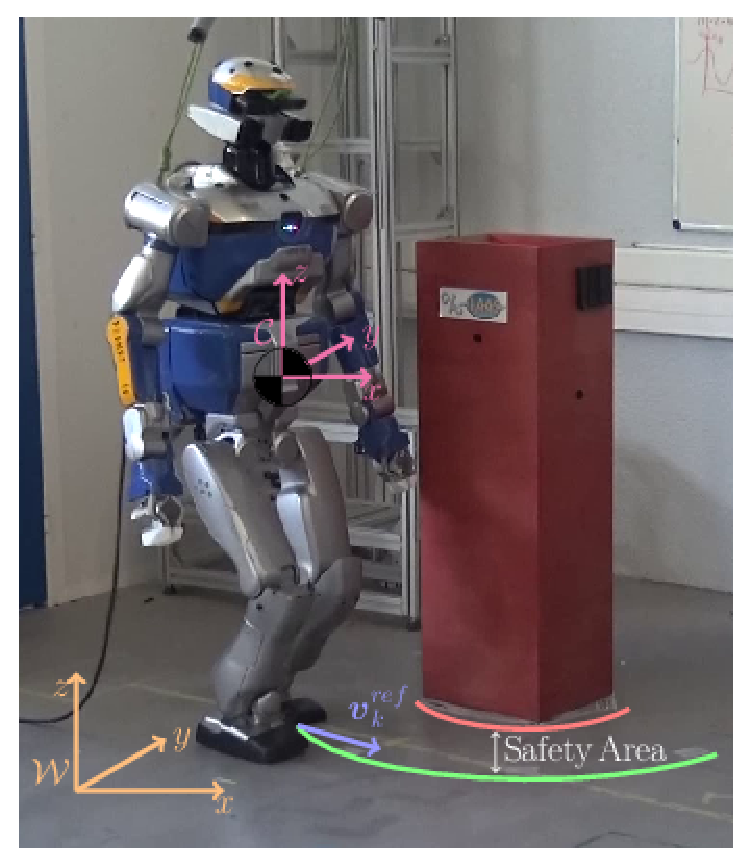
\includegraphics[width=0.7\linewidth, keepaspectratio]{./figures/synthesis}
%  \caption{HRP-2 is following an ellipse according the one-third power law. The center of gravity $\mathcal C$ is expressed in a global reference frame $\mathcal W$}
  \begin{tikzpicture}%[show background grid]% every node/.style={draw,outer sep=0pt,thick}]

% SoT
\draw [fill=green,opacity=.2,text opacity=1] (-1.5,2.2) rectangle (13.0,-2.2);
\node at(6,-2.0) {\textcolor{green!20!black!100}{Stack of Tasks}};

% Ellispe Reference
\node[rectangle,minimum width=2cm, minimum height=1cm,draw=blue!70,fill=blue!20] (ellipseref) at (4.0,3.25) {};
\node[ellipse,draw=blue,thick,minimum width=1cm,minimum height=0.5cm] at (ellipseref) {};
\node at ([yshift=-0.8cm]ellipseref) {Reference trajectory};

% Vector Field
\node[rectangle,minimum width=2cm, text width=2cm,minimum height=1cm,draw=blue!70,fill=blue!20,align=center] (vectorfields) at (0.0,0.0) 
{Vector Field\\
\includegraphics[scale=0.1]{two_third/Fig3e_EllipseBetaThird.pdf}
};
%\node at (0.0,2.5) {$\gamma,\beta$};

% Walking Pattern Generator
\node[rectangle,minimum width=2cm, minimum height=1cm,draw=blue!70,fill=blue!20]  (wpg) at (5.4,1.0) {Walking Pattern Generator};

% Task
\node[rectangle,minimum width=2cm, text width=3cm, align=center, minimum height=1cm,draw=blue!70,fill=blue!20] (ttt) at (11,1.0) 
{  Tasks for\\
   Trajectory\\
   Tracking};

% Solver
\node[rectangle,minimum width=2cm, text width=3cm, align=center, minimum height=1cm,draw=blue!70,fill=blue!20] (qp) at (11,-1.0) 
{ HQP Solver };

% Power Law
\node[rectangle,text width=2cm,align=center,minimum width=2cm, minimum height=1cm,draw=blue!70,fill=blue!20] (powerlaw) at (3.0,-1.0) {Power Law\\$\gamma,\beta$};
\path[->,>=stealth',draw=black] (vectorfields.314)-- node[below] {$\kappa$} (powerlaw.189);
\path[->,>=stealth',draw=black] (powerlaw.170)-- node[above] {$v$} (vectorfields.325);

% Robot
\node[rectangle,minimum width=2cm, minimum height=1cm,draw=blue!70,fill=blue!20] (robot) at (11,-3.5) {Robot};

% Localization
\node[rectangle,minimum width=2cm, minimum height=1cm,draw=blue!70,fill=blue!20] (localization) at (0.0,-3.5) {Localization};

%\path[->,>=stealth',draw=black] (0.0,2.25)-- (vectorfields.90);

% Links
\draw[->,>=stealth',draw=black] (ellipseref.180) -| (vectorfields.90);
\draw[->,>=stealth',draw=black] (vectorfields.42) -- node[above] {${\bf c}^*$} (wpg.180);
\path[->,>=stealth',draw=black] (wpg)-- node[above] {
$\begin{matrix}
{c}_{ref}\\{\bf z}_{ref}\\{\bf LF}_{ref}\\{\bf RF}_{ref}
\end{matrix} $
}(ttt);
\path[->,>=stealth',draw=black] (ttt)-- node[right] {\small Tasks} (qp);
\path[->,>=stealth',draw=black] (qp)-- node[xshift=0.2cm,yshift=-0.2cm,] {${\bf q}$} (robot);
\path[->,>=stealth',draw=black] (robot)-- node[below,font=\small] {Motion capture}(localization);
\path[->,>=stealth',draw=black] (localization)-- node[left] {${\bf w}$}(vectorfields);

\end{tikzpicture}

  \caption[Control scheme using the one third power law on HRP-2]{Power law based closed-loop control. An ellipse reference trajectory is specified and used, together with the power law defined by the velocity gain factor $\gamma$ and $\beta$ exponent constants, to generate the reference vector field. $(x,y,\theta)$ define the position and orientation of a frame attached to the robot's center of mass. The reference vector field defines center of mass velocity ${\bf c}^*=[\dot{x},\dot{y},\dot{\theta}]$ for the walking pattern generator. This particular walking pattern generator provides reference trajectories for the balanced center of mass ${\bf c}_{ref}$, the associated center of pressure ${\bf z}_{ref}$, and the feet ${\bf LF}_{ref},{\bf RF}_{ref}$. A whole body motion generator uses the reference trajectories to generate a command ${\bf q}$ realized by the robot (for HRP-2, this is the configuration vector). The localization component uses position measurements to provide a position ${\bf w} \in SE(3)$ of the robot, that again is used as input to the vector field to provide the correcting velocity vector ${\bf c}^*$. This chapter shows that the closed-loop approach reduces motion drifts, but not entirely, and suggests that using human-like power laws may help robots to perform faster, more accurate, and more stable motion. 
}
  \label{fig:covertwothirdpowerlaw}
\end{figure}

\subsection{Power laws governing human motion}
The speed of human motion is characterized by the one-third power law behavior;
movement speed $v$ decreases when curvature $\kappa$ increases,
following the quantitative relation $\vv = \gamma \kappa^{-\beta}$,
with $\gamma$ the piecewise constant velocity gain factor and $\beta=1/3$ the exponent.
This law, often termed the two-thirds power law due to equivalent formulation determining
angular speed $A = \gamma \kappa^{2/3}$, was first found for drawing hand motion \cite{lacquaniti_law_1983}.

Power law behaviors appear to emerge from jerk minimization \cite{huh_spectrum_2015}. Alternatively, the specific one-third power law, which is equivalent to moving with a constant equi-affine speed \cite{FlashHandzel1996}, may result from equi-affine metrics used by the human brain \cite{flash_affine_2007}, possibly in a mixture with Euclidean and full affine metrics \cite{bennequin_movement_2009}. 

Tuned to perception of biological motion, the human visual system perceives one-third power law motion as uniform, rather than movement with constant speed \cite{viviani_biological_1992}. Coupling between the motor and visual systems in the human brain is supported by stronger and more widespread brain activation patterns \cite{dayan_neural_2007}, and greater event-related desynchronization \cite{meirovitch_alpha_2015}, occurring when subjects watch one-third power law motion, compared with other power law motions.  Even imagined movements slow down in curved regions according to the one-third power law \cite{papaxanthis_relation_2012,karklinsky_timing_2015}. 
These evidences suggest that humans will perceive a humanoid robot moving according to the one-third power law as more human-like, finding his motions more predictable and easier to follow.

\subsection{Guiding trajectories for humanoid robots}
Planning humanoid robot locomotion is classically accomplished by constructing an optimal sequence of footstep transitions,
taken from a discrete set of possibilities,
that is kept small to allow reasonable computation time \cite{Chestnutt:2010:MPHR,Hornung:ICHR:12}.
The limitations of this approach in restricted scenarios yield an alternative approach; planning a reference trajectory which allows generation of the needed contacts \cite{perrin:iros:2011}.
This reference trajectory is usually generated considering balance constraints and geometrical constraints such as feasibility and manipulability. 
This approach significantly reduces the burden on the motion planner, but raises the demand for controllers capable of finding footsteps or contacts in real time.
Planning general contacts is still a very hard problem \cite{Escande:RAS:2013}, and finding a center of mass trajectory for a given set of contacts was only recently accomplished \cite{carpentier:hal-01203507}. For the restricted case of walking on flat ground, several new approaches \cite{deits:ichr:14,naveau:ral:2016,herdt:iros:2010} allow automatic finding of footstep positions. Therefore, it is now possible to move a humanoid robot by providing only a reference trajectory \cite{naveau:ral:2016, herdt:iros:2010}.

In the current study, we attempt to robustly regulate the walking motion on flat floor given a planned reference trajectory. A stable regulation process is important for correcting drifts, that appear due to the interaction of the humanoid robot's soles with the ground \cite{stasse:iros:2006}. The closed-loop control does reduce the drift. However, in this study we observe that the speed profile of the reference trajectory is crucial. The naive approach of close-loop regulation to obtain constant reference speed is unsatisfactory for HRP-2; a steady-state error is still apparent. Speed modulation according to the one-third power law nullifies this drift entirely.



\subsection{Robust trajectories with contracting dynamics}
Contracting dynamics provide a robust control policy for generating motion patterns; in presence of bounded noise exponential time convergence to a limit cycle or point is guaranteed \cite{lohmiller_contraction_1998}. By mapping an attractor of a contracting dynamical system to a movement primitive, Giese et al.~\cite{giese_realtime_2009} suggested a general control method for high dimensional systems. In robotics, contraction was already used for robust synchronization of phases of control pattern generators \cite{seo_cpg_2010} as well as for learning a set of dynamic motion primitives \cite{Perk2006}. 
In this work, we show how contracting dynamics are useful to robustly generate kinematic power law behavior. 
